% =============================================================================
% Section 4.2: System Architecture
% =============================================================================

\section{System Architecture}
\label{sec:sys-arch}

\subsection{High-Level Architecture Block Diagram}
\label{subsec:arch-block-diagram}

Figure~\ref{fig:system-arch} presents the layered architecture of NexaLearn following the Dependency Rule of Clean Architecture. The outermost layer (Presentation) handles HTTP concerns through NestJS controllers, guards, pipes, and interceptors. The Application layer contains use-case interactors that orchestrate domain objects without depending on infrastructure. The Domain layer holds entities, aggregates, value objects, domain events, and repository port interfaces in pure TypeScript with zero framework dependencies. The Infrastructure layer implements the repository ports using Prisma, Stripe SDK, Mux SDK, Redis client, and AWS S3 SDK. A shared Events module provides the transactional outbox publisher and the in-process event bus.

\begin{figure}[H]
  \centering
  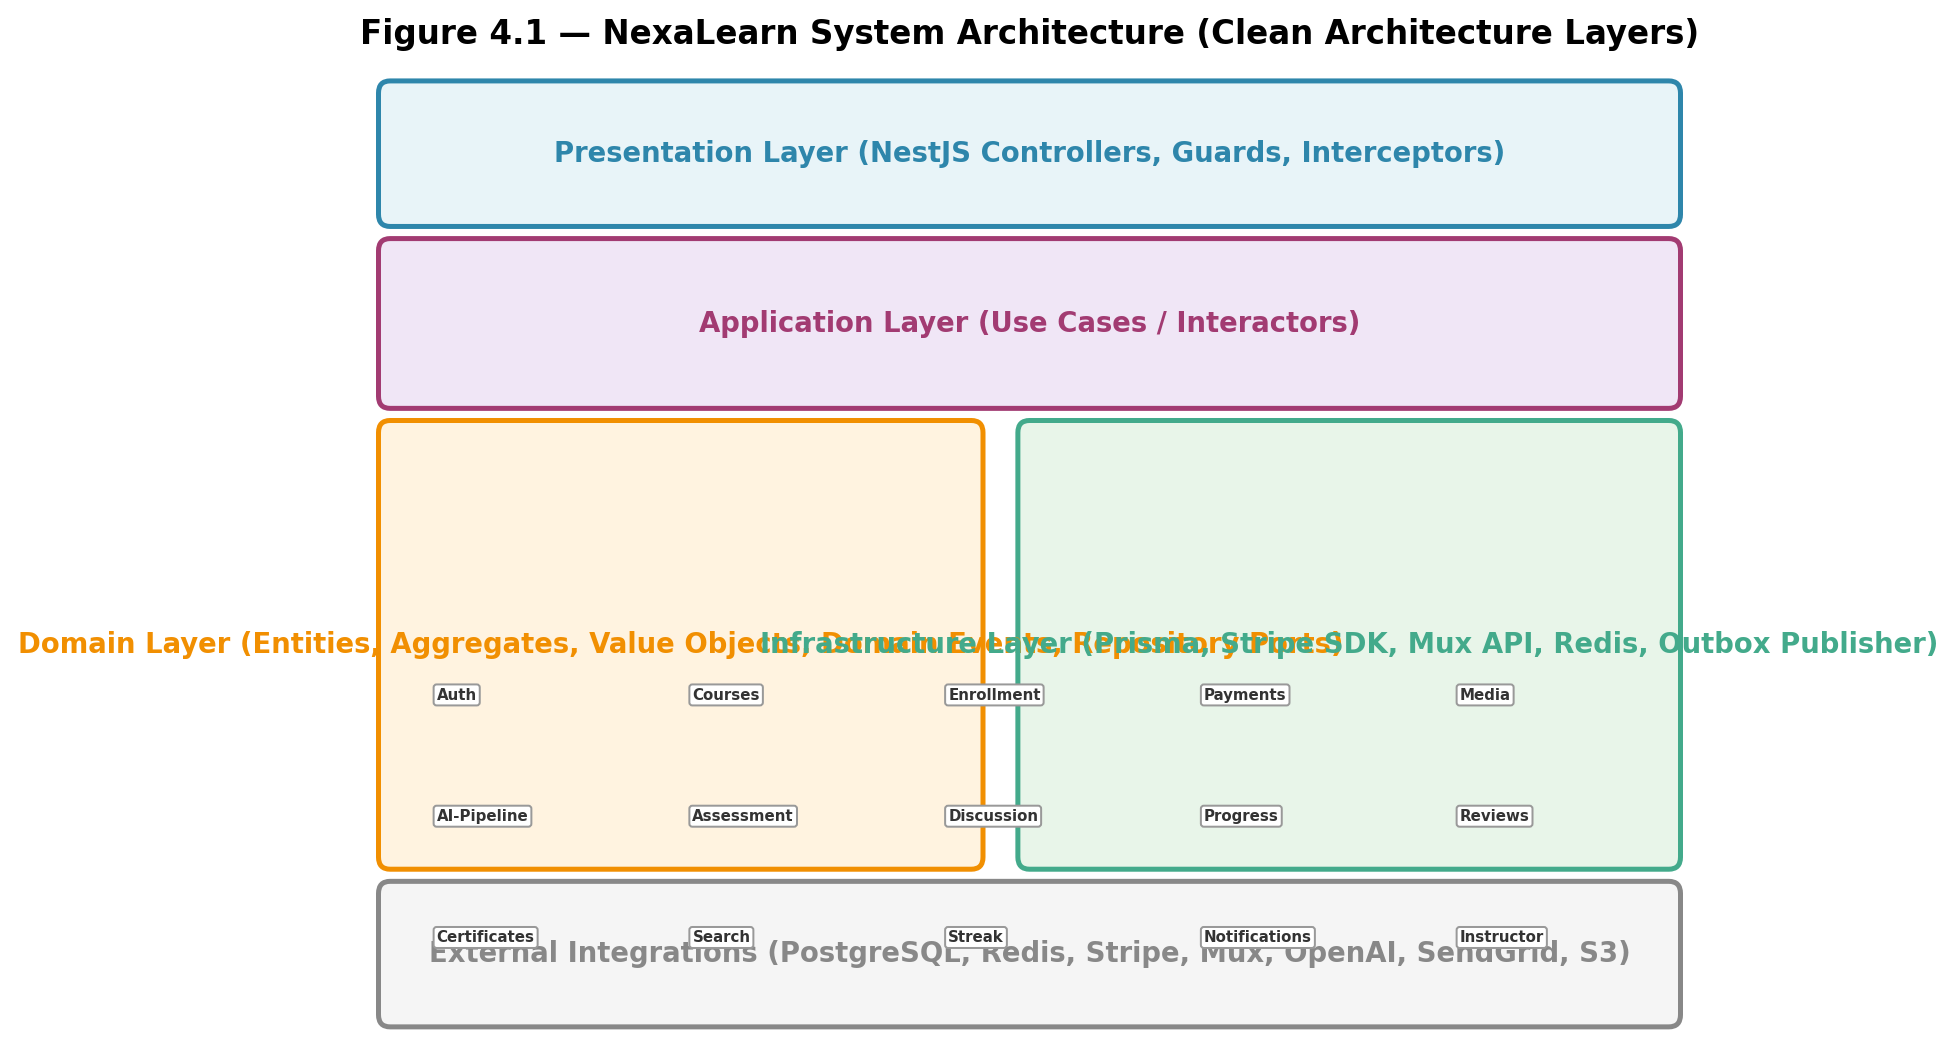
\includegraphics[width=\textwidth]{images/system_arch.png}
  \caption{NexaLearn System Architecture --- Clean Architecture Layers}
  \label{fig:system-arch}
\end{figure}

The Presentation layer routes HTTP requests to the appropriate Application use case. For example, a POST request to \texttt{/api/enrollments} is received by \texttt{EnrollmentController}, validated by a NestJS \texttt{ValidationPipe} using class-validator DTOs, and delegated to \texttt{CreateEnrollmentUseCase}. The use case loads the relevant domain aggregates (Course, User), enforces business rules (course is published, user is not already enrolled), creates a new \texttt{Enrollment} aggregate, and persists it through an \texttt{EnrollmentRepository} port. The repository implementation in Infrastructure writes to PostgreSQL via Prisma and---within the same transaction---inserts an outbox event for \texttt{EnrollmentCreated}. The outbox processor subsequently publishes this event to downstream consumers (Progress, Notifications, Search).

\subsection{Module Dependency Graph}
\label{subsec:module-dependency}

Figure~\ref{fig:module-interaction} shows the dependency and event-flow relationships among the fifteen bounded contexts. Solid arrows represent direct method-call dependencies (use cases in one context invoking repository or query service interfaces exported by another). Dashed arrows represent event-driven communication through the outbox: the source context publishes an event that is consumed by the target context's event handler.

\begin{figure}[H]
  \centering
  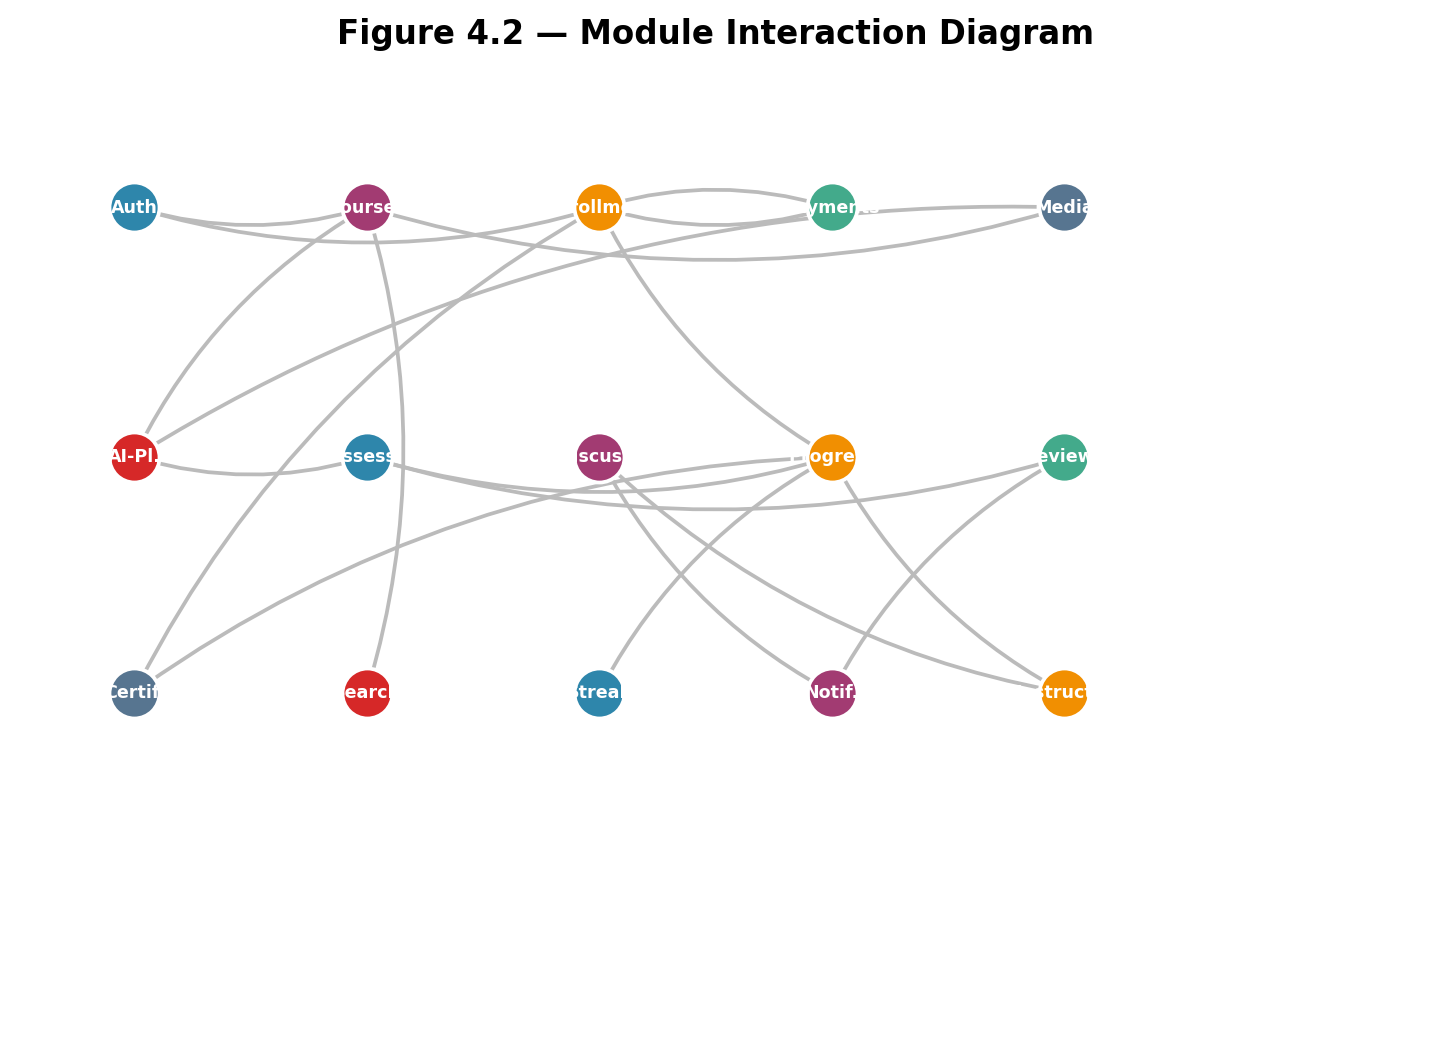
\includegraphics[width=0.8\textwidth]{images/module_interaction.png}
  \caption{NexaLearn Module Interaction Diagram}
  \label{fig:module-interaction}
\end{figure}

The diagram reveals several structural patterns. \textbf{Enrollment} acts as a hub, depending on Payments for payment verification and on Progress for projection initialisation. \textbf{Courses} depends on Media for video asset management and on AI-Pipeline for transcript and quiz generation. \textbf{Assessment} publishes graded-quiz events consumed by Progress and Reviews. \textbf{Notifications} is a pure consumer: it subscribes to events from Discussion, Reviews, and AI-Pipeline without exposing any outward-facing dependencies. \textbf{Instructor/Analytics} is a read-heavy context that queries read models built by Progress, Assessment, and Streak, and has no write-side dependencies.

\subsection{Module Summary}
\label{subsec:module-summary}

Table~\ref{tab:module-summary} enumerates all fifteen bounded contexts with their primary entities, published events, and module dependencies. This table serves as a quick reference for the detailed module descriptions that follow in Sections~\ref{sec:auth-module} through~\ref{sec:discussion-module}.

\begin{longtable}{@{}p{2.0cm} p{1.8cm} p{3.2cm} p{3.2cm} p{2.8cm}@{}}
  \caption{Module Summary --- Bounded Contexts, Entities, Events, and Dependencies}
  \label{tab:module-summary} \\
  \toprule
  \textbf{Module} & \textbf{Context} & \textbf{Key Entities} & \textbf{Key Events} & \textbf{Depends On} \\
  \midrule
  \endhead
  \midrule
  \endfoot
  Auth & Auth & User, RefreshTokenSession & UserLoggedIn, UserLoggedOut, SessionRevoked & --- \\
  \addlinespace
  Courses & Courses & Course, CourseModule, Lesson, Category & CoursePublished, LessonUpdated, CourseArchived & Media, AI-Pl. \\
  \addlinespace
  Enrollment & Enrollment & Enrollment, EnrollmentEvent & EnrollmentActivated, EnrollmentCancelled, EnrollmentCompleted & Payments, Courses \\
  \addlinespace
  Payments & Payments & PaymentIntent, PaymentTransaction, Refund & PaymentSucceeded, PaymentFailed, PaymentRefunded & Stripe (ext.) \\
  \addlinespace
  Media & Media & VideoAsset, UploadUrl, PlaybackToken & VideoUploaded, VideoReady, VideoErrored & Mux (ext.) \\
  \addlinespace
  AI-Pipeline & AI-Pipeline & GenerationJob, Transcript, GeneratedQuiz & JobCompleted, CallbackReceived, QuizReadyForReview & Media, OpenAI (ext.) \\
  \addlinespace
  Assessment & Assessment & Quiz, Question, QuestionOption, QuizAttempt, ShortAnswerGrade & QuizAttemptSubmitted, AttemptGraded, QuizPublished & Courses, AI-Pl. \\
  \addlinespace
  Discussion & Discussion & Thread, Post, ThreadInstructorReply & ThreadCreated, PostAdded, InstructorReplied & --- \\
  \addlinespace
  Progress & Progress & CourseProgressView, LessonProgress, ResumeView, LessonAnalytics & ProgressUpdated, LessonCompleted, StreakUpdated & Enrollment, Assessment \\
  \addlinespace
  Reviews & Reviews & Review, ReviewVote & ReviewSubmitted, ReviewFlagged & Assessment \\
  \addlinespace
  Certificates & Certificates & Certificate, CertificateTemplate & CertificateIssued, CertificateRevoked & Enrollment, Progress \\
  \addlinespace
  Search & Search & CourseSearchIndex, LessonSearchIndex & SearchIndexUpdated & Courses \\
  \addlinespace
  Streak & Streak & StreakRecord, StreakMilestone & StreakIncremented, StreakMilestoneReached & Progress \\
  \addlinespace
  Notifications & Notifications & Notification, EmailTemplate, NotificationPreference & NotificationSent, EmailDelivered, EmailBounced & Auth, Discussion, Assessment, Payments \\
  \addlinespace
  Instructor & Instructor & InstructorAnalyticsView, InstructorDashboard & --- (read-only) & Progress, Assessment, Streak \\
  \bottomrule
\end{longtable}

The next eight sections examine the core modules---Auth, Courses, Media, AI-Pipeline, Assessment, Payments, Enrollment, and Discussion---in architectural depth. Each section includes the domain aggregate design, state machine diagram, key code listings, and the design trade-offs that shaped the implementation.
